% ═════════════════════════════════════════════════════════════
\phantomsection
\chapter{Methodology}
\label{sec:methodology}

The pipeline of this thesis is the composition of three mathematical maps. From a raw labelled inertial recording it first produces an orientation-invariant scalar window, then a finite point cloud in $\R^m$ obtained by a delay embedding, then a fixed-length vector $\phi_\lambda(w)\in\R^{24}$ obtained by persistent homology and a small set of signal-level statistics. The vector is fed to a probabilistic classifier $f_\theta\colon\R^{24}\to[0,1]$ whose threshold determines a binary decision. The methodology specifies each of these maps, the algebraic and geometric machinery they rely on, the hyperparameter selection rule that fixes the open parameters, and the evaluation protocols under which subject-aware performance is reported. The treatment is deliberately mathematical: the central object of study is the representation map $\phi_\lambda$, not the engineering of any particular sensor pipeline, and the role of the methodology section is to make that map and its surrounding inferential framework precise.

Section~\ref{subsec:formal} fixes the formal problem setting and the principal notational conventions. Section~\ref{subsec:signal_rep} develops signal preprocessing. Section~\ref{subsec:embedding} constructs the delay embedding and states the embedding theorems of Takens and of Sauer--Yorke--Casdagli on which the geometric interpretation rests. Section~\ref{subsec:topological_prelim} recalls the necessary point-set and combinatorial topology. Section~\ref{subsec:homology} develops simplicial homology rigorously, including the fundamental identity $\partial^2=0$, the Euler--Poincar\'e formula, and the functoriality of $H_k(\,\cdot\,;\F)$. Section~\ref{subsec:ph} develops persistent homology as a functor on filtrations, including the structure theorem and the algebraic stability theorem. Section~\ref{subsec:vectorization} specifies the vectorisation. Section~\ref{subsec:classifiers} treats the two classifier families and the Platt calibration. Section~\ref{subsec:bayesopt} develops the Bayesian hyperparameter search and the tree-structured Parzen estimator. Section~\ref{subsec:eval_framework} fixes the evaluation protocols. Section~\ref{subsec:stat_inference} fixes the statistical-inference machinery. Section~\ref{subsec:compute} records the computational environment.

% ═════════════════════════════════════════════════════════════
\section{Formal Problem Setting}
\label{subsec:formal}

Let $K\in\{\mathrm{MobiFall},\,\mathrm{SisFall},\,\mathrm{FAD\_40Hz}\}$ index one of the three benchmark datasets. Each dataset consists of labelled inertial recordings together with subject identifiers, drawn from an unknown joint distribution
\[
  (\X_K,\,\Y_K,\,\Sset_K)\sim \Prob_K,
\]
where $\X_K$ is the recording-valued random element, $\Y_K\in\{0,1\}$ the binary fall label, and $\Sset_K$ the subject index, taking values in a finite set of cardinality $|\Sset_K|$. The marginal class prior $\pi_K:=\Prob_K(\Y_K=1)$ is strictly between $0$ and $1/2$ for every $K$, reflecting the empirical fact that falls are minority events.

\subsection{Resampled discrete signal}

After resampling to the target frequency $f_s=50$~Hz (justified in Section~\ref{subsubsec:rate}), a single recording is the discrete signal
\[
  \mathbf{x}\colon \{0,1,\ldots,T\}\longrightarrow\R^p,\qquad p=2,
\]
where the two coordinates are the accelerometer and gyroscope magnitudes, defined in Section~\ref{subsubsec:smv}. A binary label $y\in\{0,1\}$ indicates whether the recording contains a fall. A subject index $s\in\Sset_K$ records the individual to whom the signal belongs. The subject-aware nature of the data set is essential: independence of training and test samples is asserted at the level of subjects, not at the level of individual windows.

\subsection{Window operator}

For a window length $L\in\N$ and a starting index $t_0\in\{0,\ldots,T-L\}$, the \emph{window operator} extracts a contiguous segment:
\begin{equation}
  W_{t_0,L}\colon\R^{(T+1)\times p}\longrightarrow\R^{L\times p},
  \qquad
  W_{t_0,L}(\mathbf{x})=(\mathbf{x}_{t_0},\,\mathbf{x}_{t_0+1},\,\ldots,\,\mathbf{x}_{t_0+L-1}).
  \label{eq:window-op}
\end{equation}
The window length is determined by a hyperparameter $w_{\mathrm{sec}}>0$ measuring window duration in seconds:
\[
  L:=\lfloor w_{\mathrm{sec}}\cdot f_s\rfloor.
\]

\subsection{The hyperparameter tuple}

The topological feature extractor depends on a hyperparameter tuple
\begin{equation}
  \lambda=\bigl(w_{\mathrm{sec}},\;m,\;\tau,\;r,\;c,\;d_{\mathrm{met}},\;\varepsilon,\;q\bigr)\in\Lambda,
  \label{eq:lambda}
\end{equation}
where $w_{\mathrm{sec}}$ is the window length in seconds, $m\geq 2$ the embedding dimension, $\tau\geq 1$ the embedding lag, $r\geq 1$ the stride factor, $c\in\{\mathrm{Alpha},\,\mathrm{Rips},\,\mathrm{SparseRips}\}$ the filtered complex family, $d_{\mathrm{met}}$ a metric on $\R^m$, $\varepsilon\in(0,1)$ a filtration-scale percentile, and $q$ a subsampling rule used by the SparseRips construction. The search space $\Lambda$ is a finite Cartesian product, specified in Section~\ref{subsubsec:bayes-search-space}.

\subsection{Representation map and classifier}

Given a window $w$, the pipeline constructs a finite point cloud
\[
  P_\lambda(w)\subset\R^m
\]
by the delay embedding of Definition~\ref{def:delay} below, builds the filtered simplicial complex $\mathcal{K}_\lambda(P_\lambda(w))$ specified by $c$, computes the persistent homology in degrees $k\in\{0,1\}$, and vectorises the resulting diagrams together with a small set of signal-level features into a fixed feature vector
\begin{equation}
  \phi_\lambda(w)\in\R^{24}.
  \label{eq:phi-lambda}
\end{equation}
The dimension is fixed at $24$ regardless of $\lambda$ so that distinct configurations are compared under a uniform classifier interface.

A probabilistic classifier is a map
\[
  f_\theta\colon\R^{24}\longrightarrow[0,1],
\]
where $f_\theta(\phi_\lambda(w))$ is interpreted as the posterior probability $\widehat\Prob(\Y=1\mid w;\theta,\lambda)$. The model class is restricted to the two families
\[
  \Fcal_{\mathrm{lr}}=\{\text{balanced logistic regression models with } \ell_1\text{ or } \ell_2\text{ penalty}\},
\]
\[
  \Fcal_{\mathrm{svm}}=\{\text{balanced } C\text{-SVM models with Platt-calibrated probabilities}\}.
\]
This restriction is methodological. The aim is to test the predictive value of the representation $\phi_\lambda$ in the linear regime, not to maximise score by increasing classifier complexity.

For a threshold $\tau_0\in(0,1)$ the \emph{subject-general decision rule} is
\begin{equation}
  \widehat y(w)=\1\bigl\{f_\theta(\phi_\lambda(w))\geq\tau_0\bigr\}.
  \label{eq:dec-general}
\end{equation}
The default value of $\tau_0$ in primary evaluations is not the nominal $0.5$ but the
PR-curve optimal threshold $\hat\tau_0$ identified on the training fold; its precise
construction is described in §\ref{subsubsec:threshold}.

For subject-personalised evaluation a subject-specific threshold $\tau_s$ is used:
\begin{equation}
  \widehat y_s(w)=\1\bigl\{f_\theta(\phi_\lambda(w))\geq\tau_s\bigr\}.
  \label{eq:dec-personal}
\end{equation}
The personalised threshold $\tau_s$ must be estimated from data disjoint from the segment of subject $s$ on which the metric is finally reported; otherwise the protocol is contaminated by leakage.

\subsection{Performance functional}

The primary metric is the $F_\beta$-score evaluated at $\beta=2$,
\begin{equation}
  F_2(\widehat y,\,y)\;=\;5\,\frac{\Prec\cdot\Rec}{4\Prec+\Rec},
  \label{eq:F2-def}
\end{equation}
with $\Prec,\Rec$ computed on the test sample. The training and selection protocol prioritises recall over precision, which is the appropriate objective for fall detection when false-negative cost exceeds false-positive cost; the asymmetry is quantified in Section~\ref{subsubsec:metric}.

% ═════════════════════════════════════════════════════════════
\section{Signal Representation}
\label{subsec:signal_rep}

\subsection{Orientation invariance: the signal magnitude vector}
\label{subsubsec:smv}

A three-axis inertial sensor outputs a vector-valued signal $\mathbf{x}(t)=(x_1(t),x_2(t),x_3(t))^\top\in\R^3$. The numerical values of the axis components depend on the orientation of the device frame relative to the body frame, an SO(3)-rotation that varies across subjects and even across sessions for a fixed subject. An axis-wise representation therefore conflates motion content with nuisance orientation.

\begin{definition}[Signal magnitude vector]
\label{def:smv}
The \emph{signal magnitude vector} of a three-axis signal $\mathbf{x}\colon\Z_{\geq 0}\to\R^3$ is the scalar process
\begin{equation}
  \mathrm{SMV}(t)=\|\mathbf{x}(t)\|_2=\sqrt{x_1(t)^2+x_2(t)^2+x_3(t)^2}.
  \label{eq:smv}
\end{equation}
\end{definition}

\begin{proposition}[$\mathrm{SO}(3)$-invariance]
\label{prop:smv-invariance}
For every rotation $\mathbf{R}\in\mathrm{SO}(3)$ and every $t\geq 0$, $\|\mathbf{R}\mathbf{x}(t)\|_2=\|\mathbf{x}(t)\|_2$. Hence the map $\mathbf{x}\mapsto\mathrm{SMV}$ is invariant under reorientation of the sensor frame.
\end{proposition}

\begin{proof}
$\|\mathbf{R}\mathbf{x}\|_2^2=\mathbf{x}^\top\mathbf{R}^\top\mathbf{R}\mathbf{x}=\mathbf{x}^\top\mathbf{x}=\|\mathbf{x}\|_2^2$, using $\mathbf{R}^\top\mathbf{R}=I$.
\end{proof}

The accelerometer and the gyroscope are processed independently, producing two scalar time series $\mathrm{SMV}_{\mathrm{acc}}$ and $\mathrm{SMV}_{\mathrm{gyr}}$ per recording. All subsequent analysis is carried out on these scalar processes; the loss of directional information is the cost of orientation invariance.

\subsection{Common sampling rate}
\label{subsubsec:rate}

The three benchmark datasets were originally recorded at different rates: $87.5$~Hz (MobiFall), $200$~Hz (SisFall), and $40$~Hz (FAD\_40Hz). All signals are resampled to the common rate $f_s=50$~Hz before any further processing. The choice of $50$~Hz rests on three independent arguments.

\paragraph{Spectral sufficiency.} The fall-discriminative content of inertial wearable signals is concentrated below $20$~Hz. The pre-impact acceleration peak and the impact transient are dominated by frequencies in the $0$--$15$~Hz band; energy above $20$~Hz consists predominantly of high-frequency sensor noise and mechanical vibration~\parencite{sisfall,fallalld,kangas2008fall}.

\begin{theorem}[Nyquist--Shannon~\parencite{shannon1949communication}]
\label{thm:nyquist}
A real-valued continuous-time signal whose Fourier transform is supported in $[-B,B]$ is exactly recovered from its samples taken at any rate $f_s\geq 2B$.
\end{theorem}

With $B=20$~Hz, the rate $f_s=50$~Hz exceeds $2B=40$~Hz by a margin of $25\%$. The corresponding Nyquist frequency $f_s/2=25$~Hz dominates the relevant signal bandwidth, so resampling does not erase any fall-relevant spectral information.

\paragraph{Integer divisibility.} For SisFall the conversion ratio $200{:}50=4{:}1$ is an integer, so resampling reduces to decimation by a factor of four. For FAD\_40Hz the ratio is $40{:}50=4{:}5$ and for MobiFall the ratio is $87.5{:}50=7{:}4$; in both cases the rational ratio admits a finite-impulse-response polyphase resampler at moderate cost.

\paragraph{Computational tractability.} The persistent homology computation dominates the cost of the pipeline; on the Vietoris--Rips complex the worst-case complexity is super-polynomial in the size of the point cloud (Section~\ref{subsubsec:reduction}). A five-second window contains $L=250$ samples at $50$~Hz versus $L=1000$ samples at $200$~Hz; the resulting reduction in computational load is what makes a $200$-iteration Bayesian search across three datasets feasible.

\subsection{Window extraction}
\label{subsubsec:windows}

The classification unit is a fixed-length window of $L=\lfloor w_{\mathrm{sec}}\cdot f_s\rfloor$ samples. Fall and non-fall trials are windowed by different rules to reflect the structural difference between their respective signal regimes.

For a fall trial $\mathbf{x}$, a single window is extracted around the index of the global SMV maximum:
\begin{equation}
  t^*=\argmax_{t}\,\mathrm{SMV}_{\mathrm{acc}}(t),\qquad
  w^*=W_{t^*-\lfloor L/2\rfloor,\,L}(\mathbf{x}).
  \label{eq:fall-window}
\end{equation}
The centring strategy guarantees that the impact transient is contained in the window regardless of the recording length.

For an ADL trial, consecutive non-overlapping windows of length $L$ are extracted from the start of the recording with stride $L$:
\begin{equation}
  w_j=W_{jL,\,L}(\mathbf{x}),\qquad j=0,1,\ldots,\lfloor T/L\rfloor-1.
  \label{eq:adl-window}
\end{equation}
This produces multiple windows per ADL trial, which is appropriate because daily activities are quasi-stationary and substantially longer than fall events.

\subsection{Standard scaling}
\label{subsubsec:scaling}

After the feature vector $\phi_\lambda(w)\in\R^{24}$ has been computed for every window, each of its coordinates is centred and rescaled. Let $\mathcal{Z}=\{\phi_\lambda(w_i)\}_{i\in\mathcal{I}_{\mathrm{tr}}}\subset\R^{24}$ be the collection of feature vectors over the training partition. The empirical mean and variance per coordinate are
\[
  \mu_j=\frac{1}{|\mathcal{I}_{\mathrm{tr}}|}\sum_{i\in\mathcal{I}_{\mathrm{tr}}}\phi_\lambda(w_i)_j,
  \qquad
  \sigma_j^2=\frac{1}{|\mathcal{I}_{\mathrm{tr}}|}\sum_{i\in\mathcal{I}_{\mathrm{tr}}}\bigl(\phi_\lambda(w_i)_j-\mu_j\bigr)^2,
\]
and the standardised feature vector is $z_j=(\phi_\lambda(w)_j-\mu_j)/\sigma_j$. The parameters $\{\mu_j,\sigma_j\}$ are estimated from the training partition only and applied to the test partition; this protocol avoids information leakage from held-out subjects or windows into the normalisation procedure.

% ═════════════════════════════════════════════════════════════
\section{Phase-Space Reconstruction via Delay Embedding}
\label{subsec:embedding}

\subsection{Definition}
\label{subsubsec:delay_def}

\begin{definition}[Delay embedding]
\label{def:delay}
Let $s=(s_0,s_1,\ldots,s_{L-1})\in\R^L$ be a finite scalar sequence. For integers $m\geq 2$ (embedding dimension), $\tau\geq 1$ (lag), and $r\geq 1$ (stride), the \emph{$(m,\tau,r)$-delay embedding} of $s$ is the finite point cloud
\begin{equation}
  P_{m,\tau,r}(s)=\bigl\{\mathbf{p}_i\in\R^m:i=0,1,\ldots,N-1\bigr\},
  \label{eq:delay-emb}
\end{equation}
where
\[
  \mathbf{p}_i=\bigl(s_{ir},\,s_{ir+\tau},\,s_{ir+2\tau},\,\ldots,\,s_{ir+(m-1)\tau}\bigr),
\]
and $N=\lfloor(L-(m-1)\tau-1)/r\rfloor+1$ is the number of embedded points.
\end{definition}

Each point $\mathbf{p}_i$ collects $m$ samples of $s$ separated by lag $\tau$, and consecutive points are separated by stride $r$. As $i$ increases the sliding window traces a discrete trajectory in $\R^m$. The cardinality $N$ scales linearly in $L$ and inversely in $r$, which is decisive for the computational cost of the subsequent homology computation.

\begin{figure}[!ht]
\centering
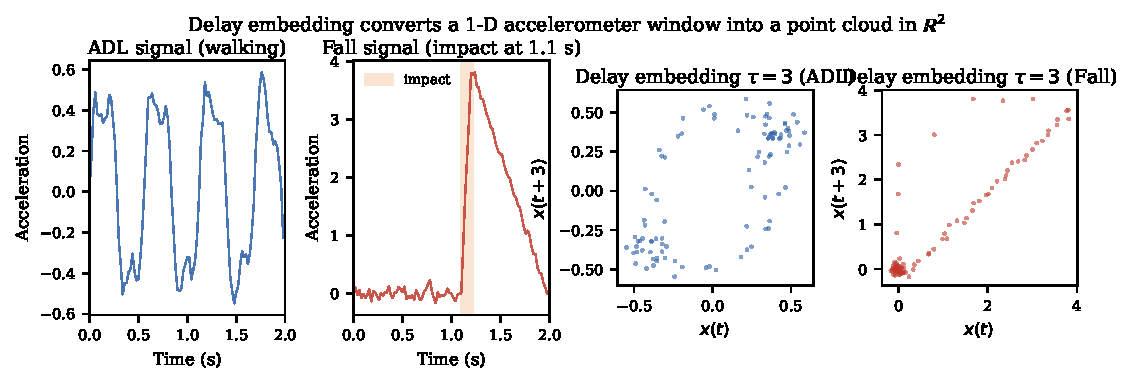
\includegraphics[width=\textwidth]{figures/fig_delay_embedding}
\caption{Left: synthetic ADL (walking) and fall accelerometer windows. Right: the
  corresponding two-dimensional delay embeddings ($m=2$, $\tau=3$).  The ADL
  trajectory forms a compact, roughly periodic arc; the fall trajectory produces a
  sparser, elongated point cloud due to the large-amplitude impact spike.  This
  geometric difference motivates the use of persistent homology to distinguish the
  two signal classes.}
\label{fig:delay-embedding}
\end{figure}

\subsection{The Takens embedding theorem}
\label{subsubsec:takens}

The use of delay coordinates is motivated by a foundational theorem of dynamical systems theory. Let $M$ be a smooth compact $d$-dimensional manifold and $\Phi\colon M\to M$ a smooth diffeomorphism (the time-$\Delta t$ flow map of an autonomous dynamical system). Let $h\colon M\to\R$ be a smooth scalar observable. The associated \emph{delay map} of order $m$ is
\[
  \Psi^{h,\Phi}_m\colon M\longrightarrow\R^m,
  \quad
  x\longmapsto\bigl(h(x),h(\Phi(x)),h(\Phi^2(x)),\ldots,h(\Phi^{m-1}(x))\bigr).
\]

\begin{theorem}[Takens~\parencite{takens1981detecting}]
\label{thm:takens}
Let $M$ be a smooth compact $d$-dimensional manifold. For $m\geq 2d+1$, it is a generic property of the pair $(\Phi,h)$ that $\Psi^{h,\Phi}_m\colon M\to\R^m$ is a smooth embedding, i.e., a smooth injective immersion onto its image. In particular, $\Psi^{h,\Phi}_m(M)$ is a smooth $d$-dimensional submanifold of $\R^m$ diffeomorphic to $M$.
\end{theorem}

\emph{Generic} means that the set of pairs $(\Phi,h)$ for which the conclusion fails is contained in a meagre subset of $C^k(M,M)\times C^k(M,\R)$ in the appropriate $C^k$-topology, i.e., a countable union of nowhere-dense sets. Theorem~\ref{thm:takens} states that, for $m$ sufficiently large relative to the intrinsic dimension of the attractor, the reconstructed trajectory is topologically and differentially faithful to the underlying state space; topological invariants computed on $P_{m,\tau,r}(s)$ therefore reflect intrinsic properties of the dynamical system that produced the signal.

\begin{theorem}[Fractal extension, Sauer--Yorke--Casdagli~\parencite{sauer1991embedology}]
\label{thm:syc}
Let $A\subseteq\R^N$ be a compact invariant set of a dynamical system with box-counting (Minkowski) dimension $\dim_B(A)=d_A$. For $m>2d_A$, almost every pair $(\Phi,h)$ (with respect to prevalence in $C^k(\R^N,\R^N)\times C^k(\R^N,\R)$) gives an injective delay map $\Psi^{h,\Phi}_m$ on $A$.
\end{theorem}

Theorem~\ref{thm:syc} relaxes the smooth-manifold assumption of Theorem~\ref{thm:takens}: fractal invariant sets, which are typical for real chaotic systems, can be embedded provided $m$ exceeds twice their box-counting dimension. This is the relevant statement for inertial sensor signals, whose attractors need not be smooth manifolds.

\begin{remark}[Heuristic status]
\label{rem:heuristic}
Theorems~\ref{thm:takens} and~\ref{thm:syc} require (i) a deterministic underlying dynamical system, (ii) infinite observation, and (iii) generic observable and dynamics. Wearable fall signals satisfy none of these hypotheses strictly: they are finite, noisy, and not the deterministic output of an autonomous flow on a fixed manifold. The theorems are therefore applied in a \emph{heuristic} rather than a rigorous sense: they motivate the use of delay coordinates as a geometrically richer representation than the raw scalar sequence, without guaranteeing that the resulting point cloud faithfully reconstructs any specific attractor. The parameters $(m,\tau,r)$ are treated as hyperparameters and selected empirically by the search of Section~\ref{subsec:bayesopt}.
\end{remark}

\subsection{Geometric interpretation for fall detection}
\label{subsubsec:geometry}

The geometric content of the delay embedding is what makes it useful for fall detection.

During a \emph{fall}, the SMV signal undergoes a brief high-amplitude transient: a sharp pre-impact rise, a peak at ground contact, and a partial decay. In the reconstruction space the trajectory makes a rapid excursion into an extreme region and does not return to its starting neighbourhood within the window. The resulting point cloud is \emph{elongated and non-recurrent}: a one-dimensional or quasi-one-dimensional sweep with few or no closed loops.

During a \emph{daily activity} such as walking, the SMV signal is approximately periodic with period $T_{\mathrm{walk}}\approx 1$~s. In the reconstruction space the trajectory traces a structured, roughly periodic orbit. The corresponding point cloud is \emph{recurrent and loop-forming}.

This structural dichotomy is precisely the geometry detected by persistent homology in degrees $k=0$ and $k=1$. The zeroth-degree summary $H_0$ records connected components; the first-degree summary $H_1$ records independent one-dimensional cycles. Fall windows are expected to exhibit pronounced $H_0$ behaviour (cluster spread along the excursion) and weak $H_1$ behaviour; ADL windows are expected to exhibit richer $H_1$ structure. The empirical statistics tabulated in Section~\ref{subsec:vectorization} are designed to quantify these expectations.

\subsection{Filtration scale control}
\label{subsubsec:eps}

For the Rips and SparseRips families, the filtration is truncated at a data-adaptive scale to bound the size of the simplicial complex. Define the multiset of inter-point distances
\[
  D(P)=\bigl\{d_{\mathrm{met}}(\mathbf{p},\mathbf{p}'):\mathbf{p},\mathbf{p}'\in P,\;\mathbf{p}\neq\mathbf{p}'\bigr\}
\]
and set
\begin{equation}
  \varepsilon_{\max}=\mathrm{Quantile}_q(D(P)),
  \qquad
  q\in\{0.20,0.40,0.60,0.80\}.
  \label{eq:eps_max}
\end{equation}
The percentile $q$ controls the scale at which the filtration is truncated: a low percentile concentrates the analysis on fine-scale local geometry; a high percentile admits coarser global structure at the cost of additional simplices. The Alpha complex requires no such cutoff because its size is intrinsically polynomial in $|P|$ via the Delaunay triangulation.

% ═════════════════════════════════════════════════════════════
\section{Topological Preliminaries}
\label{subsec:topological_prelim}

The persistent homology of the filtration depends on objects from point-set and algebraic topology that are not standard in signal processing. This section establishes the necessary background.

\subsection{Topological spaces and homotopy}

\begin{definition}[Topological space]
\label{def:topspace}
A \emph{topological space} is a pair $(X,\mathcal{T})$ where $X$ is a set and $\mathcal{T}\subseteq 2^X$ is a family of subsets, the \emph{open sets}, satisfying
\begin{enumerate}[label=(\roman*)]
  \item $\emptyset\in\mathcal{T}$ and $X\in\mathcal{T}$;
  \item $\mathcal{T}$ is closed under arbitrary unions;
  \item $\mathcal{T}$ is closed under finite intersections.
\end{enumerate}
A map $f\colon(X,\mathcal{T}_X)\to(Y,\mathcal{T}_Y)$ is \emph{continuous} if $f^{-1}(U)\in\mathcal{T}_X$ for every $U\in\mathcal{T}_Y$. A continuous bijection with continuous inverse is a \emph{homeomorphism}, written $X\cong Y$.
\end{definition}

Every metric space $(X,d)$ carries the \emph{metric topology}, generated by the open balls $B(x,r)=\{y\in X:d(x,y)<r\}$.

\begin{definition}[Homotopy and homotopy equivalence]
\label{def:homotopy}
Continuous maps $f,g\colon X\to Y$ are \emph{homotopic} ($f\simeq g$) if there exists a continuous map $H\colon X\times[0,1]\to Y$ with $H(\cdot,0)=f$ and $H(\cdot,1)=g$. A continuous map $f\colon X\to Y$ is a \emph{homotopy equivalence} if there exists $g\colon Y\to X$ with $g\circ f\simeq\mathrm{id}_X$ and $f\circ g\simeq\mathrm{id}_Y$. A space is \emph{contractible} if it is homotopy equivalent to a point.
\end{definition}

Homotopy equivalence is strictly coarser than homeomorphism. Every convex subset of $\R^m$ is contractible (via the straight-line homotopy to any interior point). Homology is a homotopy invariant: $X\simeq Y$ implies $H_k(X;\F)\cong H_k(Y;\F)$ for all $k\geq 0$.

\subsection{Abstract and geometric simplicial complexes}

\begin{definition}[Abstract simplicial complex]
\label{def:simplicial-abstract}
Let $V$ be a finite set. An \emph{abstract simplicial complex} on $V$ is a collection $K\subseteq 2^V\setminus\{\emptyset\}$ closed under non-empty subset: $\sigma\in K$ and $\emptyset\neq\rho\subseteq\sigma$ imply $\rho\in K$. An element $\sigma\in K$ with $|\sigma|=k+1$ is a \emph{$k$-simplex} of dimension $k$. The \emph{$k$-skeleton} of $K$ is $K^{(k)}=\{\sigma\in K:\dim\sigma\leq k\}$.
\end{definition}

\begin{definition}[Standard $k$-simplex]
\label{def:standard-simplex}
The \emph{standard $k$-simplex} is
\[
  \Delta^k=\conv\{e_0,e_1,\ldots,e_k\}
  =\Bigl\{(t_0,\ldots,t_k)\in\R^{k+1}:t_i\geq 0,\;\sum_{i=0}^kt_i=1\Bigr\},
\]
where $\{e_i\}$ is the standard basis of $\R^{k+1}$. Its open interior is $\mathrm{int}(\Delta^k)=\{t\in\Delta^k:t_i>0\;\forall i\}$.
\end{definition}

\begin{definition}[Geometric realisation]
\label{def:geo-real}
Let $K$ be an abstract simplicial complex with vertex set $V$. An injection $\iota\colon V\hookrightarrow\R^N$ is in \emph{general position} for $K$ if no $d+2$ vertices lie in a common affine subspace of dimension $\leq d=\dim K$. The \emph{geometric realisation} of $K$ is
\[
  |K|=\bigcup_{\sigma\in K}\conv\bigl\{\iota(v):v\in\sigma\bigr\}\subset\R^N,
\]
equipped with the subspace topology of $\R^N$.
\end{definition}

The homeomorphism type of $|K|$ does not depend on the choice of general-position embedding. Geometric realisation is \emph{functorial}: a simplicial map $f\colon K\to L$ (a vertex map sending each simplex of $K$ to a simplex of $L$) induces a continuous map $|f|\colon|K|\to|L|$ by barycentric interpolation.

% ═════════════════════════════════════════════════════════════
\section{Simplicial Homology}
\label{subsec:homology}

Fix a field $\F$. The computational implementation uses $\F=\F_2$, the field with two elements; the algebraic framework is identical over any field, modulo orientation conventions.

\subsection{Chains and the boundary operator}

An \emph{oriented $k$-simplex} is an equivalence class $[v_0,\ldots,v_k]$ of ordered tuples of distinct vertices, modulo even permutations: $[v_{\pi(0)},\ldots,v_{\pi(k)}]=\sgn(\pi)\,[v_0,\ldots,v_k]$. Each simplex of positive dimension carries exactly two orientations; over $\F_2$, where $-1=1$, orientation is irrelevant.

\begin{definition}[Chain group]
\label{def:chains}
The \emph{$k$-th chain group} $C_k(K;\F)$ is the $\F$-vector space freely generated by the oriented $k$-simplices of $K$, with the identification $-\sigma=\bar\sigma$ for the two orientations of the same underlying simplex.
\end{definition}

\begin{definition}[Boundary operator]
\label{def:boundary}
The \emph{$k$-th boundary} $\partial_k\colon C_k(K;\F)\to C_{k-1}(K;\F)$ is the $\F$-linear map defined on basis elements by
\begin{equation}
  \partial_k\bigl([v_0,v_1,\ldots,v_k]\bigr)
  =\sum_{i=0}^k(-1)^i[v_0,\ldots,\widehat{v_i},\ldots,v_k],
  \label{eq:boundary}
\end{equation}
where $\widehat{v_i}$ denotes omission of $v_i$.
\end{definition}

\begin{lemma}[Fundamental relation $\partial^2=0$]
\label{lem:boundary-squared}
For all $k\geq 1$, $\partial_{k-1}\circ\partial_k=0$.
\end{lemma}

\begin{proof}
It suffices to verify the identity on a basis element $\sigma=[v_0,\ldots,v_k]$. Two applications of \eqref{eq:boundary} give
\begin{multline*}
  \partial_{k-1}(\partial_k\sigma)
  =\sum_{j<i}(-1)^{i+j}[v_0,\ldots,\widehat{v_j},\ldots,\widehat{v_i},\ldots,v_k]\\
  +\sum_{i<j}(-1)^{i+j-1}[v_0,\ldots,\widehat{v_i},\ldots,\widehat{v_j},\ldots,v_k],
\end{multline*}
where in the second sum the omitted vertex $v_j$ has been shifted by one position because $v_i$ with $i<j$ was already deleted. For each unordered pair $\{i,j\}$ with $i<j$ the two contributions cancel exactly, yielding zero.
\end{proof}

Geometrically, Lemma~\ref{lem:boundary-squared} expresses the fact that the boundary of a simplex is itself a closed surface and hence has no boundary.

\subsection{Homology groups and Betti numbers}

Lemma~\ref{lem:boundary-squared} implies $\im(\partial_{k+1})\subseteq\ker(\partial_k)$. The quotient is well defined.

\begin{definition}[Homology and Betti numbers]
\label{def:homology}
The \emph{cycle group} is $Z_k=\ker\partial_k\subseteq C_k(K;\F)$; the \emph{boundary group} is $B_k=\im\partial_{k+1}\subseteq Z_k$. The \emph{$k$-th homology} is the quotient
\[
  H_k(K;\F)=Z_k/B_k,
\]
and the \emph{$k$-th Betti number} is $\beta_k=\dim_\F H_k(K;\F)$.
\end{definition}

The Betti numbers admit elementary geometric interpretations. $\beta_0$ counts the connected components of $|K|$; $\beta_1$ counts the number of independent one-dimensional cycles (loops not bounding any 2-chain); $\beta_2$ counts the number of enclosed two-dimensional voids.

\begin{theorem}[Euler--Poincar\'e formula]
\label{thm:euler}
Let $f_k=|\{\sigma\in K:\dim\sigma=k\}|$. The Euler characteristic of $K$, defined by
\[
  \chi(K)=\sum_{k\geq 0}(-1)^k f_k,
\]
satisfies
\begin{equation}
  \chi(K)=\sum_{k\geq 0}(-1)^k\beta_k.
  \label{eq:euler}
\end{equation}
\end{theorem}

\begin{proof}
The rank--nullity theorem applied to $\partial_k$ gives $\dim C_k=\dim Z_k+\dim B_{k-1}$ for all $k\geq 0$, with $B_{-1}=0$. Summing with alternating signs and rearranging telescopes the boundary-group terms; the result is~\eqref{eq:euler}.
\end{proof}

The formula links a combinatorial datum ($f_k$) to homotopy invariants ($\beta_k$) and serves as a consistency check on any homology computation.

\subsection{Functoriality}

\begin{definition}[Simplicial and chain maps]
\label{def:simplicial-map}
A \emph{simplicial map} $f\colon K\to L$ is a vertex map $f\colon V(K)\to V(L)$ with $f(\sigma)\in L$ for every $\sigma\in K$. The induced \emph{chain map} $f_\#\colon C_k(K;\F)\to C_k(L;\F)$ is defined on basis elements by
\[
  f_\#([v_0,\ldots,v_k])=
  \begin{cases}
    [f(v_0),\ldots,f(v_k)] & \text{if } f(v_0),\ldots,f(v_k)\text{ are distinct,}\\
    0 & \text{otherwise.}
  \end{cases}
\]
\end{definition}

One checks that $f_\#\partial_k^K=\partial_k^L f_\#$, i.e., chain maps commute with boundaries. Consequently, $f_\#$ maps cycles to cycles and boundaries to boundaries, and descends to a well-defined linear map
\[
  H_k(f)\colon H_k(K;\F)\longrightarrow H_k(L;\F),\quad [z]\longmapsto[f_\#(z)].
\]
Composition is preserved, $H_k(g\circ f)=H_k(g)\circ H_k(f)$, and identities are preserved, $H_k(\mathrm{id})=\mathrm{id}$. In categorical language, $H_k(\,\cdot\,;\F)$ is a functor from the category of simplicial complexes to the category $\Vect_\F$ of $\F$-vector spaces.

This functoriality is the bridge to persistent homology. The inclusions $K_i\hookrightarrow K_j$ for $i\leq j$ in any filtration are simplicial maps, and the induced maps $H_k(K_i;\F)\to H_k(K_j;\F)$ are the structure maps of the persistence module defined below.

% ═════════════════════════════════════════════════════════════
\section{Persistent Homology}
\label{subsec:ph}

\subsection{Filtrations and complex families}
\label{subsubsec:filtration}

\begin{definition}[Filtration]
\label{def:filtration}
A \emph{filtration} of a simplicial complex $K$ is a nested family of subcomplexes
\[
  \emptyset=K_0\subseteq K_1\subseteq\cdots\subseteq K_n=K,
\]
indexed by a non-decreasing real sequence $\varepsilon_0\leq\varepsilon_1\leq\cdots\leq\varepsilon_n$ of \emph{filtration values}.
\end{definition}

For a finite point cloud $P\subset\R^m$ equipped with metric $d_{\mathrm{met}}$, the methodology uses three filtered complex families.

\paragraph{Vietoris--Rips complex.}
\begin{equation}
  \mathcal{R}_\varepsilon(P)=\bigl\{\sigma\subseteq P:\diam_{d_{\mathrm{met}}}(\sigma)\leq\varepsilon\bigr\}.
  \label{eq:rips}
\end{equation}
The Rips complex is a \emph{flag complex}: every clique of its 1-skeleton is filled by a higher-dimensional simplex. The filtration is therefore determined entirely by the order in which edges appear.

\paragraph{Alpha complex.}
For the Euclidean metric, the Voronoi cell of $p\in P$ is
\[
  V_p=\bigl\{x\in\R^m:\|x-p\|_2\leq\|x-p'\|_2\;\forall p'\in P\bigr\}.
\]
The \emph{Alpha complex} is the nerve of the restricted cover $\{B(p,\varepsilon)\cap V_p\}_{p\in P}$:
\begin{equation}
  \mathcal{A}_\varepsilon(P)=\Bigl\{\sigma\subseteq P:\bigcap_{p\in\sigma}\bigl(B(p,\varepsilon)\cap V_p\bigr)\neq\emptyset\Bigr\}.
  \label{eq:alpha}
\end{equation}
$\mathcal{A}_\varepsilon(P)$ is a subcomplex of the Delaunay triangulation, hence has at most $O(|P|^{\lceil m/2\rceil})$ simplices, dramatically less than the worst-case Rips bound of $2^{|P|}$.

\paragraph{Sparse Rips complex.}
The SparseRips construction~\parencite{cavanna2015geometric} replaces $P$ by a greedy \emph{maxmin} landmark subset $L\subseteq P$: starting from an arbitrary seed, each successive landmark is the point of $P$ farthest from the existing landmarks. The persistent homology of the resulting weighted complex is provably a $(1+\varepsilon)$-approximation of that of $\mathcal{R}_\varepsilon(P)$ in the interleaving distance of Definition~\ref{def:interleaving}.

\begin{theorem}[Nerve theorem~\parencite{borsuk1948imbedding}]
\label{thm:nerve}
Let $\mathcal{U}=\{U_i\}_{i\in I}$ be a finite open cover of a paracompact space $X$ such that every non-empty finite intersection $U_{i_0}\cap\cdots\cap U_{i_p}$ is contractible. Then $|N(\mathcal{U})|\simeq X$, where $N(\mathcal{U})$ is the abstract simplicial complex with simplices $\{i_0,\ldots,i_p\}$ for which the corresponding intersection is non-empty.
\end{theorem}

The Alpha complex satisfies the hypothesis of Theorem~\ref{thm:nerve}: each $B(p,\varepsilon)\cap V_p$ is the intersection of a ball and a convex Voronoi cell, hence convex and therefore contractible, and finite intersections of convex subsets of $\R^m$ are convex and contractible. Consequently $|\mathcal{A}_\varepsilon(P)|\simeq\bigcup_{p\in P}B(p,\varepsilon)$: the Alpha complex faithfully encodes the topology of the union of balls without introducing simplices beyond the Delaunay triangulation.

\begin{figure}[!ht]
\centering
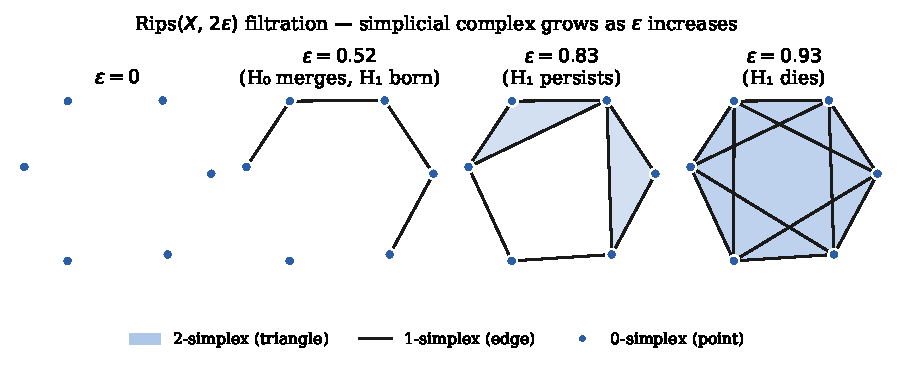
\includegraphics[width=\textwidth]{figures/fig_rips_filtration}
\caption{Rips$\,(X,2\varepsilon)$ filtration of a six-point cloud at four scales.
  At $\varepsilon=0$ only vertices are present ($\beta_0=6$, $\beta_1=0$).  As
  $\varepsilon$ increases, edges appear and connected components merge ($\beta_0$
  decreases).  A loop ($H_1$ class) is born when the polygon is complete and dies
  when triangles fill it.  Features far from the diagonal in the persistence diagram
  have long lifetime and are noise-robust (Cohen--Steiner stability,
  Theorem~\ref{thm:stability}).}
\label{fig:rips-filtration}
\end{figure}

\subsection{Persistence modules}
\label{subsubsec:persmods}

Regard the linearly ordered set $(\R,\leq)$ as a category: objects are real numbers, and there is a unique morphism $r\to s$ whenever $r\leq s$. Let $\Vect_\F$ be the category of $\F$-vector spaces and $\F$-linear maps.

\begin{definition}[Persistence module]
\label{def:persmod}
A \emph{(one-parameter) persistence module} over $\F$ is a functor
\[
  \mathbb{V}\colon(\R,\leq)\longrightarrow\Vect_\F.
\]
Concretely, $\mathbb{V}$ assigns a vector space $V_r$ to each $r\in\R$ and a linear map $\rho_{r,s}\colon V_r\to V_s$ (the \emph{structure map}) to each $r\leq s$, with $\rho_{r,r}=\mathrm{id}$ and $\rho_{s,t}\circ\rho_{r,s}=\rho_{r,t}$.
\end{definition}

A morphism $\Phi\colon\mathbb{U}\to\mathbb{V}$ is a natural transformation: linear maps $\Phi_r\colon U_r\to V_r$ with $\Phi_s\circ\rho^\mathbb{U}_{r,s}=\rho^\mathbb{V}_{r,s}\circ\Phi_r$ for all $r\leq s$. Persistence modules with such morphisms form a category $\mathbf{Pers}_\F$.

Applying $H_k(\,\cdot\,;\F)$ levelwise to a filtration and to each inclusion $K_i\hookrightarrow K_j$ yields a persistence module $\mathbb{V}_k=\{H_k(K_i;\F)\}$: the \emph{$k$-th persistence module of the filtration}. This is the central algebraic invariant studied by persistent homology.

\begin{definition}[Interleaving distance]
\label{def:interleaving}
For $\varepsilon\geq 0$, the \emph{$\varepsilon$-shift} of $\mathbb{V}$ is the persistence module $\mathbb{V}[\varepsilon]_r:=V_{r+\varepsilon}$. Modules $\mathbb{U},\mathbb{V}$ are \emph{$\varepsilon$-interleaved} if there exist morphisms $\Phi\colon\mathbb{U}\to\mathbb{V}[\varepsilon]$ and $\Psi\colon\mathbb{V}\to\mathbb{U}[\varepsilon]$ with $\Psi[\varepsilon]\circ\Phi=\rho^\mathbb{U}_{r,r+2\varepsilon}$ and $\Phi[\varepsilon]\circ\Psi=\rho^\mathbb{V}_{r,r+2\varepsilon}$ for all $r$. The \emph{interleaving distance} is
\[
  d_I(\mathbb{U},\mathbb{V})=\inf\bigl\{\varepsilon\geq 0:\mathbb{U}\text{ and }\mathbb{V}\text{ are }\varepsilon\text{-interleaved}\bigr\}.
\]
\end{definition}

The interleaving distance is an extended pseudometric on persistence modules; it descends to a metric on the set of isomorphism classes.

\subsection{The structure theorem and persistence diagrams}
\label{subsubsec:structure}

\begin{definition}[Interval module]
\label{def:interval-mod}
For $b<d$ in $\R\cup\{+\infty\}$, the \emph{interval module} $\F[b,d)$ is the persistence module with $V_r=\F$ for $b\leq r<d$, $V_r=0$ otherwise, and identity structure maps between non-zero positions.
\end{definition}

\begin{theorem}[Structure theorem, Crawley-Boevey~\parencite{crawley2015decomposition}]
\label{thm:structure}
Every pointwise finite-dimensional persistence module $\mathbb{V}$ over a field $\F$ decomposes uniquely, up to isomorphism and reordering, as a direct sum of interval modules:
\begin{equation}
  \mathbb{V}\;\cong\;\bigoplus_{i\in I}\F[b_i,d_i).
  \label{eq:structure}
\end{equation}
The multiset $\{(b_i,d_i)\}_{i\in I}$ is a complete isomorphism invariant of $\mathbb{V}$.
\end{theorem}

The special case for tame modules over filtered finite complexes was established by Zomorodian and Carlsson~\parencite{edelsbrunner2002topological}. Each interval $(b_i,d_i)$ represents a topological feature of degree $k$ that is \emph{born} at scale $b_i$ and \emph{dies} at scale $d_i$; its \emph{persistence} is $p_i=d_i-b_i$. The diagonal is added by convention so that the diagram is a multiset in
\[
  \{(b,d)\in[\,-\infty,\infty\,]^2:b\leq d\}\cup\{\text{diagonal with infinite multiplicity}\}.
\]

\begin{definition}[Persistence diagram]
\label{def:pd}
The \emph{$k$-th persistence diagram} of a filtration is
\begin{equation}
  \PD_k=\bigl\{(b_i,d_i):b_i<d_i<+\infty\bigr\}_{i\in I_k}.
  \label{eq:pd}
\end{equation}
Features with $d_i=+\infty$ are excluded from the present feature vectorisation because their infinite lifetime requires special handling in any scalar summary.
\end{definition}

\subsection{Distances and stability}
\label{subsubsec:pd-distances}

\begin{definition}[Bottleneck and Wasserstein distances]
\label{def:bottleneck}
A \emph{partial matching} between diagrams $D_1,D_2$ is a bijection $\gamma\colon D_1\cup\Delta\to D_2\cup\Delta$ that is the identity outside a finite set, where $\Delta=\{(x,x):x\in\R\}$ is the diagonal. The \emph{$p$-Wasserstein distance} ($1\leq p<\infty$) is
\[
  W_p(D_1,D_2)=\inf_\gamma\Bigl(\sum_{x\in D_1\cup\Delta}\|x-\gamma(x)\|_\infty^p\Bigr)^{1/p},
\]
and the \emph{bottleneck distance} is
\[
  d_B(D_1,D_2)=\inf_\gamma\sup_{x\in D_1\cup\Delta}\|x-\gamma(x)\|_\infty=\lim_{p\to\infty}W_p(D_1,D_2).
\]
\end{definition}

\begin{theorem}[Stability of persistence diagrams, Cohen-Steiner--Edelsbrunner--Harer~\parencite{cohen2007stability}]
\label{thm:stability}
Let $f,g\colon X\to\R$ be tame continuous functions on a triangulable compact space $X$, and let $D_f,D_g$ be the persistence diagrams of their sublevel-set filtrations. Then
\[
  d_B(D_f,D_g)\leq\|f-g\|_\infty.
\]
\end{theorem}

\begin{theorem}[Algebraic stability, Chazal et al.~\parencite{chazal2016structure}]
\label{thm:isometry}
For any two pointwise finite-dimensional persistence modules $\mathbb{U},\mathbb{V}$ over a field $\F$,
\[
  d_B\bigl(\PD(\mathbb{U}),\PD(\mathbb{V})\bigr)=d_I(\mathbb{U},\mathbb{V}).
\]
\end{theorem}

Theorem~\ref{thm:isometry} upgrades stability from an inequality to an isometry: the bottleneck distance on diagrams equals the interleaving distance on modules, providing a complete algebraic characterisation of the geometry of persistence.

For point cloud filtrations, the metric stability statement of practical interest is the following.

\begin{corollary}[Metric stability]
\label{cor:metric-stability}
Let $P,Q\subset\R^m$ be finite point sets and let
\[
  d_H(P,Q)=\max\Bigl(\max_{p\in P}\min_{q\in Q}\|p-q\|_2,\,\max_{q\in Q}\min_{p\in P}\|p-q\|_2\Bigr)
\]
be their Hausdorff distance. Then for every $k\geq 0$,
\[
  d_B\bigl(\PD_k(\mathcal{R}(P)),\,\PD_k(\mathcal{R}(Q))\bigr)\leq 2\,d_H(P,Q).
\]
\end{corollary}

\begin{proof}[Proof sketch]
If $d_H(P,Q)\leq\delta$, then each simplex of $\mathcal{R}_\varepsilon(P)$ lifts to a simplex of $\mathcal{R}_{\varepsilon+2\delta}(Q)$ by replacing each vertex by a point of $Q$ within distance $\delta$ and applying the triangle inequality to the diameter. By symmetry the two Rips modules are $2\delta$-interleaved, hence $d_B\leq 2\delta$ by Theorem~\ref{thm:isometry}.
\end{proof}

The practical content is that bounded sensor noise of amplitude $\delta$ perturbs each embedded point by at most $\delta$ in $\ell_2$, hence the persistence diagrams of two realisations of the same fall event differ by at most $2\delta$ in bottleneck distance. Features with persistence $p_i\gg 2\delta$ are noise-robust; near-diagonal features with $p_i\approx 0$ are noise-sensitive.

\begin{figure}[!ht]
\centering
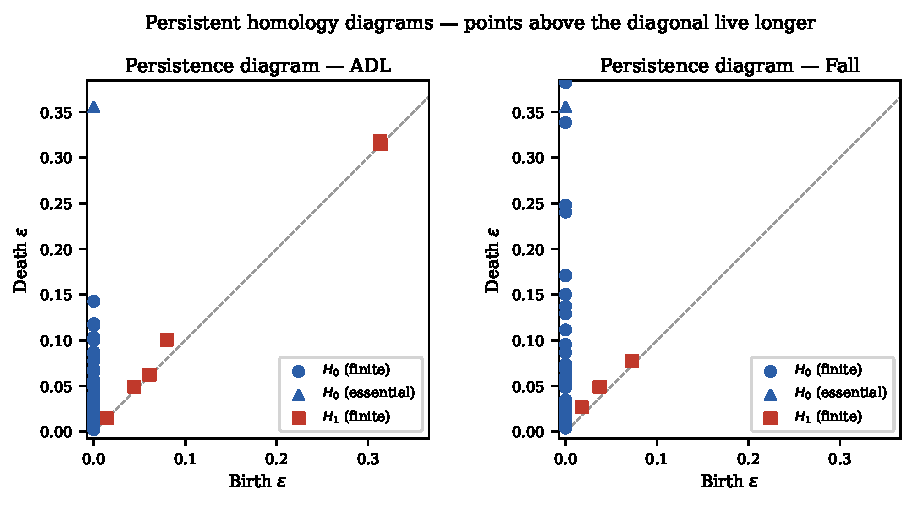
\includegraphics[width=0.85\textwidth]{figures/fig_persistence_diagram}
\caption{Persistence diagrams ($H_0$ circles, $H_1$ squares) for delay-embedded ADL
  and fall windows.  Points far from the diagonal represent long-lived topological
  features.  The fall window typically exhibits a high-persistence $H_1$ feature
  (loop) absent or short-lived in the ADL window---a geometric signature of the
  sharp impact trajectory in the delay-embedded space.  Triangles and diamonds
  denote essential classes (infinite death, plotted at the top margin).}
\label{fig:persistence-diagram}
\end{figure}

\subsection{Computational reduction}
\label{subsubsec:reduction}

Persistence diagrams are computed by \emph{boundary matrix reduction}. Order the simplices of the filtration as $\sigma_1,\sigma_2,\ldots,\sigma_n$ so that $\dim\sigma_i\leq\dim\sigma_{i+1}$ and simplices entering at smaller scale precede those at larger scale (consistent with filtration order). The boundary matrix $D\in\F^{n\times n}$ has $D_{i,j}=1$ if $\sigma_i\in\partial\sigma_j$ and $0$ otherwise. The \emph{pivot} of column $j$ is $\low(D,j)=\max\{i:D_{i,j}\neq 0\}$, undefined if column $j$ is zero.

\begin{algorithm}[H]
\caption{Standard persistence algorithm (column reduction over $\F_2$).}
\label{alg:reduction}
\begin{algorithmic}[1]
\Require Boundary matrix $D\in\{0,1\}^{n\times n}$ in filtration order
\Ensure Reduced matrix $R$ with unique pivots; persistence pairs read from $R$
\State $R\leftarrow D$
\For{$j=1$ \textbf{to} $n$}
  \While{$\exists\;i<j$ with $\low(R,i)=\low(R,j)\neq\bot$}
    \State $R[\,\cdot\,,j]\leftarrow R[\,\cdot\,,j]+R[\,\cdot\,,i]$ \Comment{column addition over $\F_2$}
  \EndWhile
\EndFor
\State \textbf{Pairs:} $\{(\low(R,j),\,j):R[\,\cdot\,,j]\neq 0\}$
\end{algorithmic}
\end{algorithm}

\begin{proposition}[Uniqueness of pairing]
\label{prop:reduction-unique}
The pairing produced by Algorithm~\ref{alg:reduction} is independent of the order in which column additions are performed; it depends only on the filtration.
\end{proposition}

The proposition is a corollary of the structure theorem~\ref{thm:structure}. The worst-case complexity of Algorithm~\ref{alg:reduction} is $O(n^3)$; the GUDHI library~\parencite{gudhi} implements optimised variants (twist reduction, clearing, dualisation to cohomology) with near-linear average-case complexity on the point cloud sizes considered here.

% ═════════════════════════════════════════════════════════════
\section{Feature Vectorisation}
\label{subsec:vectorization}

Persistence diagrams are complete isomorphism invariants of the filtration but cannot be passed directly to standard classifiers, which require fixed-length input vectors. Two obstacles obstruct direct use:
\begin{enumerate}[label=(\roman*)]
  \item the cardinality $|I_k|$ varies across windows and configurations;
  \item the diagram space, under the bottleneck or Wasserstein metric, is not a Hilbert space.
\end{enumerate}
A variety of vectorisation schemes circumvent these obstacles: persistence images~\parencite{adams2017persistence}, persistence landscapes~\parencite{bubenik2015statistical}, and others. The present methodology uses a fixed set of scalar statistics, motivated by the requirement that the feature dimension be constant across $\lambda$ to permit a uniform Bayesian search.

\subsection{Persistence-based statistics}
\label{subsubsec:stats-topo}

For each homological degree $k\in\{0,1\}$, write $\{(b_i^{(k)},d_i^{(k)})\}_{i=1}^{n_k}$ for the finite-persistence pairs of $\PD_k$, and let $p_i^{(k)}=d_i^{(k)}-b_i^{(k)}>0$ be the persistence. When $n_k=0$ all derived statistics are set to zero. Ten scalar statistics are computed per degree.

\medskip
\begin{tabular}{@{\hspace{0.3em}}clp{8.7cm}@{}}
\toprule
$j$ & Statistic & Definition \\
\midrule
1 & Bar count        & $n_k/L$ (normalised by window length) \\
2 & Entropy          & $-\sum_i\tilde p_i\log\tilde p_i,\;\tilde p_i=p_i/\sum_jp_j$ \\
3 & Maximum          & $\max_i p_i^{(k)}$ \\
4 & Energy           & $\sum_i (p_i^{(k)})^2$ \\
5 & Mean             & $\bar p^{(k)}=n_k^{-1}\sum_ip_i^{(k)}$ \\
6 & Standard dev.    & $\bigl(n_k^{-1}\sum_i(p_i-\bar p)^2\bigr)^{1/2}$ \\
7 & Median           & $Q_{0.50}(\mathbf{p}^{(k)})$ \\
8 & Q1               & $Q_{0.25}(\mathbf{p}^{(k)})$ \\
9 & Q3               & $Q_{0.75}(\mathbf{p}^{(k)})$ \\
10 & Third moment    & $n_k^{-1}\sum_i(p_i-\bar p)^3$ \\
\bottomrule
\end{tabular}
\medskip

These ten statistics for $k=0$ occupy feature positions $1$--$10$ and for $k=1$ occupy positions $11$--$20$. Together they give a 20-dimensional topological sub-vector.

\subsection{Signal-level features}
\label{subsubsec:signal-feats}

Four additional scalar features are computed directly from $\mathrm{SMV}_{\mathrm{acc}}$ on the window:
\begin{equation}
  f_{21}=\max_t\mathrm{SMV},\quad
  f_{22}=\mathrm{std}(\mathrm{SMV}),\quad
  f_{23}=\overline{\mathrm{SMV}},\quad
  f_{24}=\max_t\mathrm{SMV}-\min_t\mathrm{SMV}.
  \label{eq:sig-feats}
\end{equation}

\subsection{Complete feature vector}
\label{subsubsec:full-vec}

The complete feature vector under configuration $\lambda$ is
\begin{equation}
  \phi_\lambda(w)=\bigl(f_1^{(0)},\ldots,f_{10}^{(0)},\,f_1^{(1)},\ldots,f_{10}^{(1)},\,f_{21},f_{22},f_{23},f_{24}\bigr)\in\R^{24}.
  \label{eq:full-vec}
\end{equation}
The fixed dimension is a methodological constraint imposed by the requirement of a uniform classifier interface across $\lambda$.

% ═════════════════════════════════════════════════════════════
\section{Classification Models}
\label{subsec:classifiers}

Two linear classifier families are considered, $\Fcal_{\mathrm{lr}}$ and $\Fcal_{\mathrm{svm}}$. Both are applied with balanced class weighting and, for SVM, with Platt probability calibration.

\subsection{Logistic regression}
\label{subsubsec:lr}

Logistic regression models the conditional fall probability by
\begin{equation}
  \Prob(Y=1\mid\mathbf{z};\boldsymbol\theta,b)=\sigma(\boldsymbol\theta^\top\mathbf{z}+b),
  \qquad
  \sigma(u)=\frac{1}{1+e^{-u}},
  \label{eq:lr-sigmoid}
\end{equation}
where $\mathbf{z}\in\R^{24}$ is the standardised feature vector and $(\boldsymbol\theta,b)\in\R^{24}\times\R$ are the parameters. Given training data $\{(\mathbf{z}_i,y_i)\}_{i=1}^n$ the regularised negative log-likelihood is
\begin{equation}
  \mathcal{L}_\Omega(\boldsymbol\theta,b)
  =-\frac{1}{n}\sum_{i=1}^n\Bigl[y_i\log\sigma_i+(1-y_i)\log(1-\sigma_i)\Bigr]
  +\frac{1}{C}\,\Omega(\boldsymbol\theta),
  \label{eq:lr-loss}
\end{equation}
where $\sigma_i=\sigma(\boldsymbol\theta^\top\mathbf{z}_i+b)$, $C>0$ is the inverse regularisation strength, and $\Omega(\boldsymbol\theta)\in\{\tfrac12\|\boldsymbol\theta\|_2^2,\,\|\boldsymbol\theta\|_1\}$ selects the $\ell_2$ or $\ell_1$ penalty. The $\ell_2$ objective is strictly convex and smooth and is solved by L-BFGS or coordinate descent; the $\ell_1$ objective is convex and non-smooth and is solved by liblinear coordinate descent in the implementation.

\begin{proposition}[Convexity and uniqueness for $\ell_2$]
\label{prop:lr-convex}
With $\Omega(\boldsymbol\theta)=\tfrac12\|\boldsymbol\theta\|_2^2$, the objective~\eqref{eq:lr-loss} is strictly convex in $(\boldsymbol\theta,b)$ on $\R^{25}$, hence admits a unique global minimiser.
\end{proposition}

\begin{proof}
The negative log-likelihood is convex because $-\log\sigma(u)$ is convex in $u$ and the maps $u\mapsto\boldsymbol\theta^\top\mathbf{z}+b$ are affine. The $\ell_2$ penalty is strictly convex. The sum of a convex and a strictly convex function is strictly convex.
\end{proof}

The predicted probability is $f_\theta(\mathbf{z})=\sigma(\boldsymbol\theta^\top\mathbf{z}+b)\in(0,1)$.

\subsection{Support vector machine}
\label{subsubsec:svm}

The $C$-support vector classifier seeks a hyperplane $\{\boldsymbol{w}^\top\mathbf{z}+b=0\}$ with maximum geometric margin. With slack variables $\xi_i\geq 0$ the primal soft-margin problem is
\begin{equation}
  \min_{\boldsymbol w,b,\boldsymbol\xi}\;
  \tfrac12\|\boldsymbol w\|_2^2+C\sum_{i=1}^n\xi_i
  \quad\text{s.t.}\quad
  y_i(\boldsymbol w^\top\mathbf{z}_i+b)\geq 1-\xi_i,\;
  \xi_i\geq 0,\;
  y_i\in\{-1,+1\}.
  \label{eq:svm-primal}
\end{equation}
The Lagrangian is
\[
  L(\boldsymbol w,b,\boldsymbol\xi,\boldsymbol\alpha,\boldsymbol\mu)
  =\tfrac12\|\boldsymbol w\|^2+C\sum_i\xi_i
  -\sum_i\alpha_i\bigl[y_i(\boldsymbol w^\top\mathbf{z}_i+b)-1+\xi_i\bigr]
  -\sum_i\mu_i\xi_i,
\]
with $\alpha_i,\mu_i\geq 0$. The KKT stationarity conditions yield
\[
  \nabla_{\boldsymbol w}L=0\;\Rightarrow\;\boldsymbol w=\sum_i\alpha_iy_i\mathbf{z}_i,
  \quad
  \partial_bL=0\;\Rightarrow\;\sum_i\alpha_iy_i=0,
  \quad
  \partial_{\xi_i}L=0\;\Rightarrow\;\alpha_i+\mu_i=C.
\]
Substitution into $L$ produces the dual quadratic programme
\begin{equation}
  \max_{\boldsymbol\alpha}\;\sum_i\alpha_i-\tfrac12\sum_{i,j}\alpha_i\alpha_jy_iy_j\mathbf{z}_i^\top\mathbf{z}_j
  \quad\text{s.t.}\quad
  0\leq\alpha_i\leq C,\;\sum_i\alpha_iy_i=0.
  \label{eq:svm-dual}
\end{equation}
The primal solution recovers $\boldsymbol w^*=\sum_i\alpha_i^*y_i\mathbf{z}_i$ and the decision value for a new point is
\begin{equation}
  f(\mathbf{z})=\sum_i\alpha_i^*y_i\mathbf{z}_i^\top\mathbf{z}+b^*.
  \label{eq:svm-decision}
\end{equation}
Points with $\alpha_i^*>0$ are the \emph{support vectors}. With $\kappa(\mathbf z,\mathbf z')=\mathbf z^\top\mathbf z'$ replaced by the RBF kernel
\[
  \kappa_{\mathrm{rbf}}(\mathbf z,\mathbf z')=\exp\bigl(-\gamma\|\mathbf z-\mathbf z'\|_2^2\bigr),
\]
the same dual applies in a reproducing kernel Hilbert space.

\subsection{Platt score calibration}
\label{subsubsec:platt}

The SVM decision value $f(\mathbf z)\in\R$ is not a probability. Platt scaling~\parencite{platt1999probabilistic} fits a logistic function to the decision values on a held-out calibration set:
\begin{equation}
  \Prob(Y=1\mid\mathbf{z})=\sigma\bigl(Af(\mathbf{z})+B\bigr),
  \qquad A,B\in\R,
  \label{eq:platt}
\end{equation}
with $(A,B)$ estimated by minimising the cross-entropy loss against Laplace-smoothed targets
\[
  t_i=\begin{cases}\dfrac{n_++1}{n_++2}&\text{if }y_i=+1,\\[4pt]\dfrac{1}{n_-+2}&\text{if }y_i=-1,\end{cases}
\]
where $n_\pm$ are the counts of positive and negative calibration examples. The smoothing prevents degenerate $0$ or $1$ predictions when the margin is large.

\subsection{Class-weighted empirical risk}
\label{subsubsec:classweight}

Falls are minority events; with $n_0$ negative and $n_1$ positive training examples ($n=n_0+n_1$) the \emph{balanced class weights} are
\begin{equation}
  w_c=\frac{n}{2\,n_c},\qquad c\in\{0,1\}.
  \label{eq:cw}
\end{equation}
This satisfies $w_0n_0=w_1n_1=n/2$. For logistic regression, the weighted log-likelihood replaces $\mathcal{L}_\Omega$ by
\[
  \mathcal{L}_\Omega^{\mathrm{w}}(\boldsymbol\theta,b)
  =-\frac{1}{n}\sum_{i=1}^n w_{y_i}\Bigl[y_i\log\sigma_i+(1-y_i)\log(1-\sigma_i)\Bigr]
  +\frac{1}{C}\Omega(\boldsymbol\theta).
\]
For C-SVM, the scalar $C$ in~\eqref{eq:svm-primal} is replaced by $C_+=Cw_1$ for positive examples and $C_-=Cw_0$ for negative examples, biasing the model toward higher recall.

% ═════════════════════════════════════════════════════════════
\section{Bayesian Hyperparameter Optimisation}
\label{subsec:bayesopt}

The representation map $\phi_\lambda$ depends on the hyperparameter tuple $\lambda\in\Lambda$ of~\eqref{eq:lambda}, and the classifier depends on its own tuple $\theta\in\Theta$ (regularisation strength, penalty, kernel). Joint optimisation over $\Lambda\times\Theta$ is necessary because the two tuples interact: the geometry of the topological representation determines which classifier hyperparameters are optimal. The optimisation is performed by Bayesian search with a tree-structured Parzen estimator (TPE), implemented in Optuna~\parencite{optuna}.

\subsection{The optimisation problem}
\label{subsubsec:opt-problem}

Let $\mathcal{D}^{\mathrm{train}}_K$ be the labelled feature corpus of dataset $K$ from which the test subject has been removed (LOSO outer split, Section~\ref{subsubsec:protocols}). Let
\[
  \mathrm{CV}_K\colon\Lambda\times\Theta\longrightarrow\R,
  \qquad
  (\lambda,\theta)\longmapsto\widehat{F}_{2,K}(\lambda,\theta)
\]
denote the inner cross-validation estimator of $\E[F_2\mid K,\lambda,\theta]$ obtained by stratified $k$-fold CV on $\mathcal{D}^{\mathrm{train}}_K$. The optimisation problem solved at each outer fold is
\begin{equation}
  \lambda^*_K,\theta^*_K\;\in\;\argmax_{(\lambda,\theta)\in\Lambda\times\Theta}\mathrm{CV}_K(\lambda,\theta).
  \label{eq:bayes-objective}
\end{equation}
The objective is non-differentiable, noisy (because CV estimates fluctuate with the random fold partition and stochastic class-balancing), and expensive to evaluate (each call requires constructing point clouds, computing persistent homology, fitting the classifier, and performing the CV averaging). These properties make grid search infeasible and motivate a sequential model-based approach.

\subsection{Sequential model-based optimisation}
\label{subsubsec:smbo}

Sequential model-based optimisation (SMBO)~\parencite{hutter2011sequential} alternates between fitting a probabilistic surrogate to past evaluations and proposing new evaluations that maximise an acquisition function under the surrogate. Let $y(\lambda,\theta)=\mathrm{CV}_K(\lambda,\theta)+\eta$ denote one noisy evaluation of the objective, with $\eta$ centred. After $t$ evaluations the data set is
\[
  \mathcal{H}_t=\bigl\{((\lambda_i,\theta_i),y_i):i=1,\ldots,t\bigr\}.
\]
A surrogate $p(y\mid\lambda,\theta,\mathcal{H}_t)$ is a probability model over the objective conditional on the search point and the history. The standard acquisition function is the \emph{expected improvement} (EI) over a reference value $y^*$:
\begin{equation}
  \EI_{y^*}(\lambda,\theta)=\E\bigl[\max(y^*-y,0)\bigm|\lambda,\theta,\mathcal{H}_t\bigr].
  \label{eq:ei}
\end{equation}
(Here EI is stated for a minimisation problem with $y$ the negative $\widehat F_2$; sign conventions are equivalent under negation.) The next search point is
\begin{equation}
  (\lambda_{t+1},\theta_{t+1})\in\argmax_{(\lambda,\theta)\in\Lambda\times\Theta}\EI_{y^*}(\lambda,\theta).
  \label{eq:smbo-step}
\end{equation}
The surrogate is updated and the loop continues for a fixed budget. The textbook surrogate is a Gaussian process posterior; TPE replaces it with a non-parametric density model that is better suited to discrete and conditional search spaces.

\subsection{Tree-structured Parzen estimator}
\label{subsubsec:tpe}

TPE~\parencite{bergstra2011algorithms} models the posterior in an inverted form. Instead of modelling $p(y\mid\lambda,\theta)$ directly, it splits the observed history at a quantile $\gamma\in(0,1)$ and models the density of the inputs given two quality regimes,
\[
  p(\lambda,\theta\mid y\leq y^*)=\ell(\lambda,\theta),
  \qquad
  p(\lambda,\theta\mid y>y^*)=g(\lambda,\theta),
\]
where $y^*$ is the empirical $\gamma$-quantile of the observed $\{y_i\}$. The two density estimates are constructed from the corresponding subsets of $\mathcal{H}_t$ by kernel density estimation: each observation contributes a kernel centred at its parameter value, with bandwidth determined adaptively. Conditional and discrete hyperparameters are handled by a hierarchical tree structure on $\Lambda\times\Theta$, with each node carrying its own one-dimensional kernel.

\begin{proposition}[EI under TPE is the ratio of densities]
\label{prop:tpe-ratio}
Under the TPE generative model, the expected improvement $\EI_{y^*}(\lambda,\theta)$ is proportional to the ratio of the conditional densities:
\[
  \EI_{y^*}(\lambda,\theta)\;\propto\;\left(\gamma+\frac{g(\lambda,\theta)}{\ell(\lambda,\theta)}\,(1-\gamma)\right)^{-1}.
\]
Consequently, maximising EI is equivalent to maximising the ratio $\ell(\lambda,\theta)/g(\lambda,\theta)$.
\end{proposition}

\begin{proof}[Proof sketch]
With $p(y\leq y^*)=\gamma$, Bayes' rule gives
\[
  p(\lambda,\theta)=\gamma\,\ell+(1-\gamma)\,g,
  \qquad
  p(y\leq y^*\mid\lambda,\theta)=\frac{\gamma\,\ell}{\gamma\,\ell+(1-\gamma)\,g}.
\]
Substitution into $\EI_{y^*}=\int_{-\infty}^{y^*}(y^*-y)p(y\mid\lambda,\theta)\,dy$ and elementary manipulation yields the displayed proportionality~\parencite{bergstra2011algorithms}.
\end{proof}

\subsection{Comparison with alternative search strategies}
\label{subsubsec:alternatives}

Four search paradigms are available for the optimisation of~\eqref{eq:bayes-objective}. The
present methodology adopts TPE-SMBO; this subsection provides a quantitative justification.

\paragraph{Grid search.}
Under the conditional structure of $\Lambda$ specified in
Section~\ref{subsubsec:bayes-search-space}, the total number of distinct
configurations is
\begin{equation}
  |\Lambda_{\mathrm{grid}}|
  = n_w\cdot n_m\cdot n_\tau\cdot n_r\,
    \bigl(1 + 2\,n_d\,n_\varepsilon\bigr)
  = 9\cdot 4\cdot 5\cdot 3\cdot(1+2\cdot 4\cdot 4)
  = 17{,}820,
  \label{eq:grid-count}
\end{equation}
where the factor $1$ accounts for the Alpha branch (metric and filtration-scale parameters
inactive) and $2\cdot 16=32$ for the Rips and SparseRips branches. Combined with the
classifier grids, $|\Lambda_{\mathrm{grid}}|\times(|\Theta_{\mathrm{lr}}|+|\Theta_{\mathrm{svm}}|)
= 17{,}820\times 18 = 320{,}760$ inner-CV evaluations are needed \emph{per outer LOSO fold}.
For SisFall with $|\Sset_K|=24$ outer folds, a conservative estimate of $5$~s per inner-CV
call gives approximately
\[
  320{,}760\times 24\times 5\;\mathrm{s}\;\approx\;43\;\text{days},
\]
making full grid search computationally infeasible on the available hardware.

\paragraph{Random search.}
Random search~\parencite{bergstra2012random} draws configurations independently and uniformly
from $\Lambda\times\Theta$ without reference to past evaluations. It is
statistically consistent under infinite budget and, under the low effective-dimensionality
hypothesis, outperforms grid search at equal sample count by avoiding wasted evaluations
on uninformative axes. For the present budget $T=200$, however, random search explores
only $200/17{,}820\approx 1.1\%$ of the grid and provides no mechanism for directing
subsequent trials toward promising regions identified by earlier ones.

\paragraph{Gaussian-process Bayesian optimisation.}
The canonical SMBO surrogate is a Gaussian process (GP), which models the objective as a
GP-distributed random function and updates its posterior via Bayes' rule after each
evaluation. GP-SMBO is appropriate when the search space is a compact subset of $\R^d$
with a natural metric. It is unsuitable here for two structural reasons. First, no natural
stationary kernel is defined on the conditional, mixed-type space $\Lambda\times\Theta$
without auxiliary embeddings whose inductive bias is difficult to justify. Second, fitting
and inverting the GP covariance matrix costs $O(t^3)$ in the evaluation count $t$; for
$T=200$ iterations this overhead is non-negligible and grows quadratically with the
complexity of the correlation model.

\paragraph{TPE (adopted strategy).}
TPE~\parencite{bergstra2011algorithms} resolves both difficulties. The conditional structure of
$\Lambda$ is encoded natively in the tree; each leaf node carries an independent
univariate kernel density estimator, so per-iteration update cost is $O(t)$.
Proposition~\ref{prop:tpe-ratio} provides the theoretical guarantee that maximising
$\ell/g$ is equivalent to maximising EI under the TPE generative model. Empirically,
TPE has outperformed GP-EI on machine-learning hyperparameter benchmarks at comparable
budgets~\parencite{bergstra2011algorithms,bergstra2012random}, and its implementation in
Optuna~\parencite{optuna} handles mixed, conditional, and discrete spaces transparently.

\subsection{Search space}
\label{subsubsec:bayes-search-space}

The search space $\Lambda$ is the Cartesian product
\begin{align*}
  w_{\mathrm{sec}}&\in\{1.0,\,1.5,\,2.0,\,2.5,\,3.0,\,3.5,\,4.0,\,4.5,\,5.0\}\;\text{(s)},\\
  m&\in\{2,3,4,5\},\quad \tau\in\{1,2,3,4,5\},\quad r\in\{1,2,4\},\\
  c&\in\{\mathrm{Alpha},\,\mathrm{Rips},\,\mathrm{SparseRips}\},\\
  d_{\mathrm{met}}&\in\{\text{Euclidean, Manhattan, Chebyshev, Cosine}\},\\
  q&\in\{0.20,\,0.40,\,0.60,\,0.80\},\quad \varepsilon\in\Lambda_\varepsilon,
\end{align*}
where $\Lambda_\varepsilon$ denotes the auxiliary filtration parameter associated with $c$. Several conditional constraints are imposed by the geometry: the Alpha complex requires the Euclidean metric; metric and $q$ are inactive for the Alpha complex. The classifier search spaces are
\[
  \Theta_{\mathrm{lr}}=\bigl\{(C,\Omega):C\in\{10^{-2},10^{-1},1,10,10^2\},\;\Omega\in\{\ell_1,\ell_2\}\bigr\},
\]
\[
  \Theta_{\mathrm{svm}}=\bigl\{(C,\kappa):C\in\{10^{-1},1,10,10^2\},\;\kappa\in\{\mathrm{linear},\mathrm{rbf}\}\bigr\}.
\]
For the personal protocol of Section~\ref{subsubsec:protocols} the LR grid is reduced to $C\in\{10^{-1},1,10\}$ to mitigate overfitting in smaller per-subject training sets.

\subsection{Outer LOSO and inner cross-validation}
\label{subsubsec:nested-cv}

The selection procedure is the nested protocol
\begin{enumerate}[label=(\arabic*)]
  \item \textbf{Outer.} For each subject $s\in\Sset_K$, define $\mathcal{D}^{\mathrm{train}}_K(s)$ as the union of all windows of subjects $\Sset_K\setminus\{s\}$.
  \item \textbf{Inner.} Run TPE for $T=200$ iterations on $\mathcal{D}^{\mathrm{train}}_K(s)$ using stratified $k$-fold CV; record $\lambda^*_K(s),\theta^*_K(s)$.
  \item \textbf{Retrain and test.} Fit a final model on $\mathcal{D}^{\mathrm{train}}_K(s)$ with $(\lambda^*_K(s),\theta^*_K(s))$ and evaluate on the held-out subject $s$.
\end{enumerate}
The outer LOSO ensures that no information from the test subject is used to choose any model component; the inner CV ensures that the surrogate objective is an unbiased estimator of expected performance on unseen subjects from the training pool.

\begin{remark}[Computational budget]
\label{rem:bayes-budget}
The budget $T=200$ was chosen empirically as the smallest value at which the running best objective stabilises across independent runs of the search on the three datasets. Larger budgets do not produce reliably different optima, given the noise level of the inner CV estimator.
\end{remark}

\begin{remark}[Implementation decomposition]
\label{rem:impl-decomp}
Equation~\eqref{eq:bayes-objective} states a joint optimisation over $\Lambda\times\Theta$.
In practice this joint search is decomposed into two sequential stages to reduce
computational cost.
\emph{Stage~1 (TDA search, Optuna):} A single TPE study is run per dataset for
$T=200$ iterations.
The objective is the average $F_2$ of a logistic regression proxy and a linear SVM
proxy, both with fixed hyperparameters, evaluated by three-fold CV on a balanced
training subset.
Using lightweight proxies keeps each function evaluation fast, so the budget is spent
exploring $\Lambda$ rather than the joint space; the averaged objective ensures the
recovered $\lambda^*$ is not overfitted to a single classifier's inductive bias.
\emph{Stage~2 (classifier search, \texttt{GridSearchCV}):} Given $\lambda^*$,
classifier hyperparameters $\theta^*$ are selected by exhaustive grid search with
three-fold CV on the features extracted under $\lambda^*$.
This decomposition approximates the joint optimum while keeping computation tractable.
\end{remark}

\begin{remark}[Classifier-agnostic TDA search]
\label{rem:agnostic-search}
Rather than running a separate Optuna study for each classifier family, a single
study is run with a classifier-agnostic objective.
Define
\[
  \lambda^* \;\in\; \argmax_{\lambda\in\Lambda}\;
  \frac{1}{2}\Bigl(
    \mathrm{CV}_K^{\mathrm{LR}}(\lambda) +
    \mathrm{CV}_K^{\mathrm{SVM}}(\lambda)
  \Bigr),
\]
where $\mathrm{CV}_K^f(\lambda)$ denotes the $K$-fold cross-validated $F_2$ obtained
by classifier $f$ on features extracted under $\lambda$, with $f$'s hyperparameters
fixed at proxy values.
The averaged objective recovers a configuration $\lambda^*$ whose features support
good performance across classifier families simultaneously.
The map $\phi_{\lambda^*}\colon\R^{L\times 2}\to\R^{24}$ must therefore produce an
image that is both approximately linearly separable (beneficial for LR) and
geometrically well-structured in pairwise distance (beneficial for SVM with a
nonlinear kernel).
A representation satisfying both conditions is a stronger finding than one tuned
to a single classifier's inductive bias.
\end{remark}

% ═════════════════════════════════════════════════════════════
\section{Evaluation Framework}
\label{subsec:eval_framework}

\subsection{Performance metrics}
\label{subsubsec:metric}

Given binary predictions $\widehat y_i$ and labels $y_i$ on a test sample $\{(\widehat y_i,y_i)\}_{i=1}^N$, define the four confusion counts $\mathrm{TP},\,\mathrm{TN},\,\mathrm{FP},\,\mathrm{FN}$ and the four derived rates
\[
  \Acc=\frac{\mathrm{TP}+\mathrm{TN}}{N},
  \quad
  \Rec=\frac{\mathrm{TP}}{\mathrm{TP}+\mathrm{FN}},
  \quad
  \Prec=\frac{\mathrm{TP}}{\mathrm{TP}+\mathrm{FP}},
  \quad
  F_1=\frac{2\Prec\Rec}{\Prec+\Rec}.
\]
The principal metric is the $F_\beta$-score at $\beta=2$,
\begin{equation}
  F_2=(1+\beta^2)\frac{\Prec\cdot\Rec}{\beta^2\Prec+\Rec}\bigg|_{\beta=2}=\frac{5\Prec\Rec}{4\Prec+\Rec}.
  \label{eq:F2}
\end{equation}

\begin{proposition}[Recall weighting under $F_\beta$]
\label{prop:F2-recall-weight}
For fixed precision $\Prec=p$ and recall $\Rec=r$,
\[
  \frac{\partial F_\beta}{\partial r}\bigg|_{\beta=2}\;=\;\frac{20\,p^2}{(4p+r)^2}.
  \qquad
  \frac{\partial F_\beta}{\partial p}\bigg|_{\beta=2}\;=\;\frac{5\,r^2}{(4p+r)^2}.
\]
Consequently, near $p=r$ the marginal $F_2$-gain per unit of recall is four times the marginal gain per unit of precision.
\end{proposition}

\begin{proof}
Direct differentiation of~\eqref{eq:F2} and the substitution $p=r$ give the ratio $4$ between the two partial derivatives.
\end{proof}

The weighting ratio $4{:}1$ is a deliberate methodological choice: a missed fall leaves a vulnerable person unattended after a potentially injurious event, whereas a false alarm requires at most an unnecessary check. The $F_2$ score is used both as the Bayesian objective and as the headline metric in all result tables.

\begin{remark}[Non-triviality of the baseline]
\label{rem:f2-baseline}
A trivial all-positive classifier achieves $\Rec=1$ and $\Prec=\pi$, hence $F_2=5\pi/(4\pi+1)$. For $\pi<0.30$ in all three datasets this gives $F_2<0.56$, well below the scores reported in the Experiments section. The recall-oriented objective does not degenerate to a trivial solution.
\end{remark}

\subsection{Decision threshold}
\label{subsubsec:threshold}

A probabilistic classifier $f_\theta\colon\R^{24}\to[0,1]$ assigns each window a posterior fall probability. A binary label is produced by thresholding at the trained threshold $\hat\tau_0$,
\begin{equation}
  \widehat y(w)=\1\bigl\{f_\theta(\phi_\lambda(w))\geq\hat\tau_0\bigr\}.
  \label{eq:dec-thresh}
\end{equation}
The trained threshold $\hat\tau_0$ is the PR-curve optimal value identified on the training fold: $\hat\tau_0=\argmax_{\tau}F_2^{\mathrm{train}}(\tau)$. This PR-curve selection is performed once per LOSO fold using the training-fold probability scores and labels. The value $\hat\tau_0$ varies across subjects and datasets (typically in the range $[0.55, 0.85]$) and is more conservative than the nominal $\tau_0=0.50$ because the class-imbalanced training distribution places the optimal precision--recall trade-off above the $50\,\%$ probability level.

\subsection{Evaluation protocols}
\label{subsubsec:protocols}

Three evaluation scenarios are reported, each measuring a different level of generalisation.

\paragraph{Naive protocol.}
The feature matrix is partitioned uniformly at random into training (70\%) and test (30\%) sets with no constraint on subject membership. The same subject can contribute windows to both partitions. This protocol systematically overestimates performance on new individuals and is reported only as an upper-bound reference. Ten random partitions are used; results are reported as means.

\paragraph{General protocol (leave-one-subject-out).}
For each $s\in\Sset_K$ the test set is $\{w:\text{subject}(w)=s\}$ and the training set is the complement. This LOSO scheme directly measures generalisation to a previously unseen individual. Because the class-balancing procedure is stochastic, each fold is repeated $R=15$ times with independent random seeds; reported quantities are means or appropriate aggregates over the resulting $|\Sset_K|\times R$ collection of values. The General protocol is the principal protocol of the thesis.

\paragraph{Personal protocol.}
For each $s\in\Sset_K$ a model is trained and tested exclusively on that subject's own windows via a $70/30$ random split, repeated $R=15$ times. The personal protocol represents the idealised setting in which a per-user calibration period is available before deployment.

\paragraph{Decision-threshold sweep.}
Using the General-protocol classifier, the threshold $\tau$ is swept over the grid $\T=\{0.05,0.10,\ldots,0.95\}\subset(0,1)$ for each held-out subject. The subject-level retrospective gain is
\begin{equation}
  \Delta F_2(s)=\max_{\tau\in\T}F_2(\tau,s)-F_2(\hat\tau_0(s),s),
  \label{eq:dF2}
\end{equation}
where $\hat\tau_0(s)$ is the PR-curve trained threshold for subject $s$ (Section~\ref{subsubsec:threshold}). The average $\overline{\Delta F_2}=|\Sset_K|^{-1}\sum_s\Delta F_2(s)$ quantifies how much the PR-curve-calibrated trained threshold underperforms a subject-specific oracle. Because $\tau^*(s)=\argmax_\tau F_2(\tau,s)$ is identified on the same test windows on which it is evaluated, the sweep is a retrospective diagnostic of heterogeneity, not a valid prospective personalisation scheme.

% ═════════════════════════════════════════════════════════════
\section{Statistical Inference}
\label{subsec:stat_inference}

The statistical reporting framework distinguishes two sources of variability: the within-subject variability $V_{\mathrm{rep}}$ across the $R=15$ repetitions of the class-balancing procedure, and the across-subject variability $V_{\mathrm{subj}}$ in mean performance across the subject pool. The thesis reports these separately, in line with the methodological correction stated in the proposal: subject-level averages, dispersion, and uncertainty estimates take precedence over headline maxima.

\subsection{Repetition-level confidence intervals}
\label{subsubsec:rep-ci}

For each $(\text{subject } s,\text{repetition } j)$ pair let $x_{s,j}\in[0,1]$ denote the metric of interest (typically $F_2$). Define the per-repetition study-level mean
\[
  \bar X_j=|\Sset_K|^{-1}\sum_{s\in\Sset_K}x_{s,j},
  \qquad j=1,\ldots,R.
\]
The overall study mean is $\overline{X}_K=R^{-1}\sum_j\bar X_j$. The sample standard deviation of $\{\bar X_j\}$ is
\[
  S_R=\Bigl(\frac{1}{R-1}\sum_{j=1}^R(\bar X_j-\overline{X}_K)^2\Bigr)^{1/2}.
\]

\begin{theorem}[Repetition-level $t$ confidence interval]
\label{thm:t-ci}
If the per-repetition study means $\bar X_j$ are exchangeable and approximately Gaussian, then a $1-\alpha$ confidence interval for the limiting expectation $\E[\bar X]$ as $R\to\infty$ is
\begin{equation}
  \overline{X}_K\;\pm\;t_{\alpha/2,\,R-1}\;\frac{S_R}{\sqrt R},
  \label{eq:t-ci}
\end{equation}
where $t_{\alpha/2,R-1}$ is the upper $\alpha/2$ quantile of the $t$-distribution with $R-1$ degrees of freedom.
\end{theorem}

For $R=15$ and $\alpha=0.05$, $t_{0.025,14}\approx 2.145$. The interval~\eqref{eq:t-ci} captures the repetition-to-repetition stochastic variability of the class-balancing procedure; it does not capture subject-level heterogeneity.

\subsection{Subject-level paired tests}
\label{subsubsec:paired-tests}

Many of the central comparisons in the thesis are paired at the subject level: $F_2^{\mathrm{lr}}(s)$ vs $F_2^{\mathrm{svm}}(s)$, $F_2^{\mathrm{pers}}(s)$ vs $F_2^{\mathrm{gen}}(s)$, or $F_2$ for two distinct $\lambda$ values. Let
\[
  \delta_s=A_s-B_s\in\R,\qquad s\in\Sset_K,
\]
denote the per-subject paired difference, with the sign convention that positive $\delta_s$ favours $A$.

\begin{theorem}[Paired $t$-test]
\label{thm:paired-t}
Under the null $H_0\colon\E[\delta_s]=0$ and Gaussianity of $\{\delta_s\}$, the statistic
\[
  T_K=\frac{\bar\delta\sqrt{|\Sset_K|}}{S_\delta},
  \qquad
  \bar\delta=|\Sset_K|^{-1}\sum_s\delta_s,
  \quad
  S_\delta^2=\frac{1}{|\Sset_K|-1}\sum_s(\delta_s-\bar\delta)^2,
\]
is distributed as $t_{|\Sset_K|-1}$.
\end{theorem}

\begin{remark}[Robustness via the sign test]
\label{rem:sign-test}
When $|\Sset_K|$ is small (notably $|\Sset_K|=9$ for MobiFall) the Gaussianity assumption of Theorem~\ref{thm:paired-t} is hard to validate. As a robustness check, the thesis also reports the exact sign test on the binarised signs $\sgn(\delta_s)$, which under $H_0$ are exchangeable Bernoulli$(1/2)$ variates. The two-sided $p$-value is $2\Prob(\mathrm{Bin}(|\Sset_K|,1/2)\geq k)$ where $k=|\{s:\delta_s>0\}|$ (with the obvious correction for $\delta_s=0$).
\end{remark}

\subsection{Bootstrap confidence intervals}
\label{subsubsec:bootstrap}

For statistics whose finite-sample distribution is difficult to derive, the thesis uses the nonparametric paired bootstrap. Let $\theta(\{\delta_s\})$ denote a real-valued statistic of the paired differences (e.g., the subject mean, median, or interquartile range). Generate $B$ bootstrap resamples $\{\delta_s^{*,b}\}_{s\in\Sset_K}$ by sampling $|\Sset_K|$ subjects with replacement from $\Sset_K$ and copying their $\delta_s$ values, and compute
\[
  \theta_b^*=\theta(\{\delta_s^{*,b}\}),\quad b=1,\ldots,B.
\]
The $1-\alpha$ percentile confidence interval is
\begin{equation}
  \bigl[\theta^*_{(\alpha/2)},\,\theta^*_{(1-\alpha/2)}\bigr],
  \label{eq:bootstrap}
\end{equation}
where $\theta^*_{(p)}$ is the $p$-quantile of $\{\theta_b^*\}$. The thesis uses $B=10{,}000$ and $\alpha=0.05$. The bootstrap is the principal device for reporting uncertainty on subject-level summaries such as $\overline{\Delta_K}$ and $\Var(\Delta_{K,s})$ in the personalisation analysis.

\subsection{Permutation tests}
\label{subsubsec:permutation}

For exact small-sample inference on the sign pattern of paired differences, the thesis uses the paired sign-flipping permutation test. Under the exchangeability null
\[
  H_0\colon\;\delta_s\;\overset{d}{=}\;-\delta_s\qquad\text{for all } s,
\]
the $2^{|\Sset_K|}$ sign-flipped vectors $\{\epsilon_s\delta_s\}$ with $\epsilon_s\in\{-1,+1\}$ are exchangeable in distribution. The exact two-sided $p$-value of an observed test statistic $T_{\mathrm{obs}}=T(\delta)$ is
\begin{equation}
  p=\frac{1}{2^{|\Sset_K|}}\sum_{\epsilon\in\{-1,+1\}^{|\Sset_K|}}\1\bigl\{|T(\epsilon\odot\delta)|\geq|T_{\mathrm{obs}}|\bigr\}.
  \label{eq:permutation}
\end{equation}
For $|\Sset_K|\leq 24$ the sum is computed exactly; for larger $|\Sset_K|$ it is estimated by sampling $10{,}000$ random sign vectors.

\subsection{Distributional analysis of personalisation}
\label{subsubsec:dist-pers}

The personalisation question requires a distributional rather than a single-number answer. The proposal formulates the per-subject gain
\[
  \Delta_{K,s}=F_{2,K,s}^{\mathrm{pers}}-F_{2,K,s}^{\mathrm{gen}}.
\]
The thesis reports the four summaries
\[
  \overline{\Delta}_K,
  \qquad
  \mathrm{med}(\Delta_{K,s}),
  \qquad
  \Var(\Delta_{K,s}),
  \qquad
  \widehat{\Prob}(\Delta_{K,s}>0)
\]
together with bootstrap percentile confidence intervals of Section~\ref{subsubsec:bootstrap} for each. The thesis privileges the joint pattern of these four quantities over any single one, because personalisation is interpreted as a heterogeneous subject-level intervention rather than a constant treatment effect.

\subsection{Cross-applied hyperparameters}
\label{subsubsec:cross-applied}

To evaluate dataset-specific topological geometry, optimal tuples are cross-applied across datasets. Define the cross-applied estimator
\[
  \widehat F_2(K\mid\lambda^*_{K'})=\E\bigl[F_2\mid K,\lambda^*_{K'}\bigr],
\]
where the expectation is taken over the LOSO folds of dataset $K$ with the hyperparameter tuple optimised on a different dataset $K'\neq K$. The matrix
\[
  M_{K,K'}=\widehat F_2(K\mid\lambda^*_{K'})
\]
has diagonal entries equal to the General-protocol $F_2$ of each dataset under its own optimiser. Off-diagonal degradations
\[
  \mathrm{Drop}_{K\to K'}=M_{K,K}-M_{K,K'}
\]
quantify the cost of transplanting a hyperparameter tuple from $K$ to $K'$. The drops are reported per off-diagonal cell with bootstrap percentile intervals.

\subsection{Methodological correction over headline maxima}
\label{subsubsec:headline-correction}

Headline maxima such as the best single-subject score or the best Optuna objective are not used as the primary evidence in this thesis. The reasons are statistical. The maximum of a finite collection of noisy estimators is biased upward by the selection event; the bias scales with the number of competing candidates and the variance of each. Reporting subject means, subject-level confidence intervals, and the joint distribution of subject-level differences avoids this bias and provides estimands that are directly interpretable as expectations over the population from which the subjects were drawn.

% ═════════════════════════════════════════════════════════════
\section{Computational Infrastructure}
\label{subsec:compute}

All experiments were executed on the National HPC Centre (UHeM, Istanbul), allocation 4025462026, under the SLURM workload manager. Compute nodes were equipped with dual Intel Xeon Gold 6148 processors (2.40~GHz base clock, 20 physical cores per socket, 40 cores per node) and 190~GB of RAM. No GPU acceleration was used: the persistent homology reduction of Algorithm~\ref{alg:reduction} is intrinsically sequential at the point cloud sizes considered, and the gain of porting to GPU is dominated by the constant factor of the optimised CPU implementation.

The Bayesian optimisation ran sequentially across $T=200$ TPE trials per dataset, with $15$ parallel inner-CV workers per trial. Across the three datasets the total wall-clock time was approximately $3$~h $45$~min, with peak memory usage close to $10$~GB per node. Persistent homology was computed with the GUDHI library~\parencite{gudhi}; classification models were implemented in scikit-learn~\parencite{scikit-learn}. All randomness was seeded for reproducibility, and the seed list, the search history, and the resulting per-subject scores are archived alongside the thesis source.


